In questa appendice mostreremo un esempio completo di utilizzo di \textit{DbN}, in particolare
l'esempio n.6 dell'articolo \citetitle{ProbOfEx} \cite{ProbOfEx} con la seguente 
$ KB = (\mathcal{T},\mathcal{A}) $

$ \mathcal{T}Box $ :
\begin{itemize}
	\item[] $ Bipolar \sqsubseteq Depressed $
	\item[] $ \mathbf T(Depressed) \sqsubseteq_{0.85} \neg\exists hasSymptom.MoodReactivity $
	\item[] $ \mathbf T(Bipolar) \sqsubseteq_{0.70} \exists hasSymptom.MoodReactivity $
	\item[] $ \mathbf T(ProstateCancerPatient) \sqsubseteq_{0.60} \exists hasSymptom.MoodReactivity $
	\item[] $ \mathbf T(ProstateCancerPatient) \sqsubseteq_{0.80} \exists hasSymptom.Nocturia $
	\item[] $ \mathbf T(Depressed) \sqsubseteq_{0.60} \exists Smart $
\end{itemize}
$\mathcal{A}Box $ :
\[ \{ Depressed(Greg), \neg Smart(Greg) \} \]
Set of \textit{Symptoms} $\mathcal{V} $:
\[ \{ \exists hasSymptom.MoodReactivity(Greg) \} \]
Set of Cost of Disease with \textit{Tipicality}:
\[ \{ Bipolar: 1000, ProstateCancerPatient: 10000, Depressed: 3000 \} \]

Output dello strumento con la seguente ontologia; passo 1, 
verifica della condizione $ KB \cup \mathcal{V} \equiv $ consistente:
\begin{minted}{text}
========== Adding a set of Symptoms to the KB ==========
Sintomo aggiunto: Greg MoodReactivity
========== Checking consistency ==========
========== The ontology is consistent ==========
\end{minted}
passo 2, generazione scenari possibili:
\begin{minted}{text}
INIZIO SCENARIO 1
Typical(Bipolar),Greg,0.7
Probabilità scenario: 0.364
FINE SCENARIO 1

INIZIO SCENARIO 2
Typical(ProstateCancerPatient),Greg,0.48
Probabilità scenario: 0.144
FINE SCENARIO 2

INIZIO SCENARIO 3
Typical(Bipolar),Greg,0.7
Typical(ProstateCancerPatient),Greg,0.48
Probabilità scenario: 0.3356
FINE SCENARIO 3
\end{minted}
passo 3, per ogni scenario si effettua l'inferenza, viene mostrato il primo come esempio:

\begin{minted}{text}
ONTOLOGIA PRIMA DELLA LETTURA DELLA QUERY
Greg member_of Depressed
Greg member_of Not(Smart)
Bipolar is_a [ontoBase.Depressed, owl.Thing]
Depressed is_a [owl.Thing]
MoodReactivity is_a [owl.Thing]
ProstateCancerPatient is_a [owl.Thing]
Nocturia is_a [owl.Thing]
Smart is_a [owl.Thing]
Not(Smart) is_a [owl.Thing]
Not(MoodReactivity) is_a [owl.Thing]
Depressed1 is_a [owl.Thing, ontoBase.r1.only ...
IntersectionDepressedDepressed1 is_a [ontoBase ...
NotDepressed1 is_a [owl.Thing, ontoBase.r1.some( ...
Bipolar1 is_a [owl.Thing, ontoBase.r1.only(Not( ...
IntersectionBipolarBipolar1 is_a [ontoBase ...
NotBipolar1 is_a [owl.Thing, ontoBase.r1.some( ...
ProstateCancerPatient1 is_a [owl.Thing, ontoBase.r1.only ...
IntersectionProstateCancerPatientProstateCancerPatient1 is_a ...
NotProstateCancerPatient1 is_a [owl.Thing, ontoBase.r1.some( ...
FINE ONTOLOGIA PRIMA DELLA LETTURA DELLA QUERY

LETTURA SINTOMI
Sintomo aggiunto: Greg: Not(MoodReactivity)

TRADUCENDO LO SCENARIO: 
INIZIO SCENARIO
Bipolar,Greg,0.7; 
ProbabilitÓ scenario: 0.364
FINE SCENARIO

Membro tipico:
Greg is_a Bipolar
Greg is_a Bipolar1
Greg is_a IntersectionBipolarBipolar1
FINE TRADUZIONE SCENARIO

ONTOLOGIA CON SCENARIO E SINTOMI
Bipolar is_a [ontoBase.Depressed, owl.Thing]
Depressed is_a [owl.Thing]
MoodReactivity is_a [owl.Thing]
ProstateCancerPatient is_a [owl.Thing]
Nocturia is_a [owl.Thing]
Smart is_a [owl.Thing]
Not(Smart) is_a [owl.Thing]
Not(MoodReactivity) is_a [owl.Thing]
Depressed1 is_a [owl.Thing, ontoBase.r1.only ...
IntersectionDepressedDepressed1 is_a [ontoBase ...
NotDepressed1 is_a [owl.Thing, ontoBase.r1.some( ...
Bipolar1 is_a [owl.Thing, ontoBase.r1.only(Not( ...
IntersectionBipolarBipolar1 is_a [ontoBase ...
NotBipolar1 is_a [owl.Thing, ontoBase.r1.some( ...
ProstateCancerPatient1 is_a [owl.Thing, ontoBase.r1.only ...
IntersectionProstateCancerPatientProstateCancerPatient1 is_a ...
NotProstateCancerPatient1 is_a [owl.Thing, ontoBase.r1.some( ...
Greg member_of Depressed
Greg member_of MoodReactivity
Greg member_of Not(Smart)
Greg member_of Not(MoodReactivity)
Greg member_of Bipolar1
Greg member_of IntersectionBipolarBipolar1
FINE ONTOLOGIA CON SCENARIO E SINTOMI
=====================
Il fatto segue logicamente nel seguente scenario: 
INIZIO SCENARIO
Bipolar,Greg,0.7; 
ProbabilitÓ scenario: 0.364
FINE SCENARIO
=====================
ONTOLOGIA PRIMA DELLA LETTURA DELLA QUERY
Greg member_of Depressed
Greg member_of Not(Smart)
Bipolar is_a [ontoBase.Depressed, owl.Thing]
Depressed is_a [owl.Thing]
MoodReactivity is_a [owl.Thing]
ProstateCancerPatient is_a [owl.Thing]
Nocturia is_a [owl.Thing]
Smart is_a [owl.Thing]
Not(Smart) is_a [owl.Thing]
Not(MoodReactivity) is_a [owl.Thing]
Depressed1 is_a [owl.Thing, ontoBase.r1.only ...
IntersectionDepressedDepressed1 is_a [ontoBase ...
NotDepressed1 is_a [owl.Thing, ontoBase.r1.some( ...
Bipolar1 is_a [owl.Thing, ontoBase.r1.only(Not( ...
IntersectionBipolarBipolar1 is_a [ontoBase ...
NotBipolar1 is_a [owl.Thing, ontoBase.r1.some( ...
ProstateCancerPatient1 is_a [owl.Thing, ontoBase.r1.only ...
IntersectionProstateCancerPatientProstateCancerPatient1 is_a ...
NotProstateCancerPatient1 is_a [owl.Thing, ontoBase.r1.some( ...
FINE ONTOLOGIA PRIMA DELLA LETTURA DELLA QUERY

LETTURA SINTOMI
Sintomo aggiunto: Greg: Not(MoodReactivity)

TRADUCENDO LO SCENARIO: 
INIZIO SCENARIO
ProstateCancerPatient,Greg,0.48; 
ProbabilitÓ scenario: 0.14400000000000002
FINE SCENARIO
Membro tipico:
Greg is_a ProstateCancerPatient
Greg is_a ProstateCancerPatient1
Greg is_a IntersectionProstateCancerPatientProstateCancerPatient1

FINE TRADUZIONE SCENARIO
ONTOLOGIA CON SCENARIO E SINTOMI

Bipolar is_a [ontoBase.Depressed, owl.Thing]
Depressed is_a [owl.Thing]
MoodReactivity is_a [owl.Thing]
ProstateCancerPatient is_a [owl.Thing]
Nocturia is_a [owl.Thing]
Smart is_a [owl.Thing]
Not(Smart) is_a [owl.Thing]
Not(MoodReactivity) is_a [owl.Thing]
Depressed1 is_a [owl.Thing, ontoBase.r1.only ...
IntersectionDepressedDepressed1 is_a [ontoBase ...
NotDepressed1 is_a [owl.Thing, ontoBase.r1.some( ...
Bipolar1 is_a [owl.Thing, ontoBase.r1.only(Not( ...
IntersectionBipolarBipolar1 is_a [ontoBase ...
NotBipolar1 is_a [owl.Thing, ontoBase.r1.some( ...
ProstateCancerPatient1 is_a [owl.Thing, ontoBase.r1.only ...
IntersectionProstateCancerPatientProstateCancerPatient1 is_a ...
NotProstateCancerPatient1 is_a [owl.Thing, ontoBase.r1.some( ...
Greg member_of Depressed
Greg member_of MoodReactivity
Greg member_of ProstateCancerPatient
Greg member_of Nocturia
Greg member_of Not(Smart)
Greg member_of Not(MoodReactivity)
Greg member_of ProstateCancerPatient1
Greg member_of IntersectionProstateCancerPatientProstateCancerPatient1

FINE ONTOLOGIA CON SCENARIO E SINTOMI

=====================
Il fatto segue logicamente nel seguente scenario: 
INIZIO SCENARIO
ProstateCancerPatient,Greg,0.48; 
ProbabilitÓ scenario: 0.14400000000000002
FINE SCENARIO
=====================
ONTOLOGIA PRIMA DELLA LETTURA DELLA QUERY

Greg member_of Depressed
Greg member_of Not(Smart)
Bipolar is_a [ontoBase.Depressed, owl.Thing]
Depressed is_a [owl.Thing]
MoodReactivity is_a [owl.Thing]
ProstateCancerPatient is_a [owl.Thing]
Nocturia is_a [owl.Thing]
Smart is_a [owl.Thing]
Not(Smart) is_a [owl.Thing]
Not(MoodReactivity) is_a [owl.Thing]
Depressed1 is_a [owl.Thing, ontoBase.r1.only ...
IntersectionDepressedDepressed1 is_a [ontoBase ...
NotDepressed1 is_a [owl.Thing, ontoBase.r1.some( ...
Bipolar1 is_a [owl.Thing, ontoBase.r1.only(Not( ...
IntersectionBipolarBipolar1 is_a [ontoBase ...
NotBipolar1 is_a [owl.Thing, ontoBase.r1.some( ...
ProstateCancerPatient1 is_a [owl.Thing, ontoBase.r1.only ...
IntersectionProstateCancerPatientProstateCancerPatient1 is_a ...
NotProstateCancerPatient1 is_a [owl.Thing, ontoBase.r1.some( ...
FINE ONTOLOGIA PRIMA DELLA LETTURA DELLA QUERY

LETTURA SINTOMI
Sintomo aggiunto: Greg: Not(MoodReactivity)

TRADUCENDO LO SCENARIO: 
INIZIO SCENARIO
Bipolar,Greg,0.7; ProstateCancerPatient,Greg,0.48; 
ProbabilitÓ scenario: 0.33599999999999997
FINE SCENARIO
Membro tipico:
Greg is_a Bipolar
Greg is_a Bipolar1
Greg is_a IntersectionBipolarBipolar1
Membro tipico:
Greg is_a ProstateCancerPatient
Greg is_a ProstateCancerPatient1
Greg is_a IntersectionProstateCancerPatientProstateCancerPatient1
FINE TRADUZIONE SCENARIO

ONTOLOGIA CON SCENARIO E SINTOMI
Bipolar is_a [ontoBase.Depressed, owl.Thing]
Depressed is_a [owl.Thing]
MoodReactivity is_a [owl.Thing]
ProstateCancerPatient is_a [owl.Thing]
Nocturia is_a [owl.Thing]
Smart is_a [owl.Thing]
Not(Smart) is_a [owl.Thing]
Not(MoodReactivity) is_a [owl.Thing]
Depressed1 is_a [owl.Thing, ontoBase.r1.only ...
IntersectionDepressedDepressed1 is_a [ontoBase ...
NotDepressed1 is_a [owl.Thing, ontoBase.r1.some( ...
Bipolar1 is_a [owl.Thing, ontoBase.r1.only(Not( ...
IntersectionBipolarBipolar1 is_a [ontoBase ...
NotBipolar1 is_a [owl.Thing, ontoBase.r1.some( ...
ProstateCancerPatient1 is_a [owl.Thing, ontoBase.r1.only ...
IntersectionProstateCancerPatientProstateCancerPatient1 is_a ...
NotProstateCancerPatient1 is_a [owl.Thing, ontoBase.r1.some( ...
Greg member_of Depressed
Greg member_of MoodReactivity
Greg member_of ProstateCancerPatient
Greg member_of Nocturia
Greg member_of Not(Smart)
Greg member_of Not(MoodReactivity)
Greg member_of Bipolar1
Greg member_of IntersectionBipolarBipolar1
Greg member_of ProstateCancerPatient1
Greg member_of IntersectionProstateCancerPatientProstateCancerPatient1
FINE ONTOLOGIA CON SCENARIO E SINTOMI

Il fatto segue logicamente nel seguente scenario: 
INIZIO SCENARIO
Bipolar,Greg,0.7; ProstateCancerPatient,Greg,0.48; 
ProbabilitÓ scenario: 0.33599999999999997
FINE SCENARIO
\end{minted}

\clearpage

passo 4, elenco degli scenari verificati e relativo grafico:
\begin{minted}{text}
RISULTATI DELL'INTERROGAZIONE: 
SCENARI IN CUI LA QUERY SEGUE LOGICAMENTE
INIZIO SCENARIO 1
Bipolar,Greg,0.7; 
Probabilità complessiva dello scenario: 0.364
FINE SCENARIO 1

INIZIO SCENARIO 2
ProstateCancerPatient,Greg,0.48; 
Probabilità complessiva dello scenario: 0.14400000000000002
FINE SCENARIO 2

INIZIO SCENARIO 3
Bipolar,Greg,0.7; ProstateCancerPatient,Greg,0.48; 
Probabilità complessiva dello scenario: 0.33599999999999997
FINE SCENARIO 3

PROBABILITÀ TOTALE: 0.844

Fine simulazione, tempo totale:  1.984983205795288  s
\end{minted}

\paragraph{Analisi dei risultati} \hfill

Possiamo vedere nelle figure \ref{fig: A_web} ed \ref{fig: A_doc} una rappresentazione
grafica dei risultati finali. Iniziamo dunque descrivendo i tre assi cartesiani (due x e uno y) e il loro significato magari non immediato. L'asse x 
contiene il numero della diagnosi (1,2,3) con il suo corrispettivo istogramma e 
punto della funzione a dispersione, infatti ,sui due assi y, troviamo raffigurata sia la probabilità della diagnosi (scenario) $ t $, 
espressa in percentuale `\%`, sia il costo stimato della stessa,
espressa in €. Come rappresentazione si è scelto nel primo caso un istogramma al
cui interno troviamo
la/le malattia/e considerata/e come possibile spiegazione. 
Ogni rettangolo è identificato con colore diverso per la variabile, per darne risalto, essendo
un fattore importante che facilità la scelta 
dell'eventuale iter terapeutico. Per quanto riguarda la spesa medica si è preferito un
grafico a dispersione in quanto questo criterio decisionale è secondario alla salute del 
paziente e, soprattutto necessita ulteriori sviluppi.

In conclusione si fa notare al lettore la presenza della legenda riassuntiva e delle etichette esplicative sui relativi assi,
in particolare la probabilità complessiva delle possibili diagnosi (escluso lo scenario vuoto, cioè nessuna spiegazione).

\begin{figure}
	\centering
	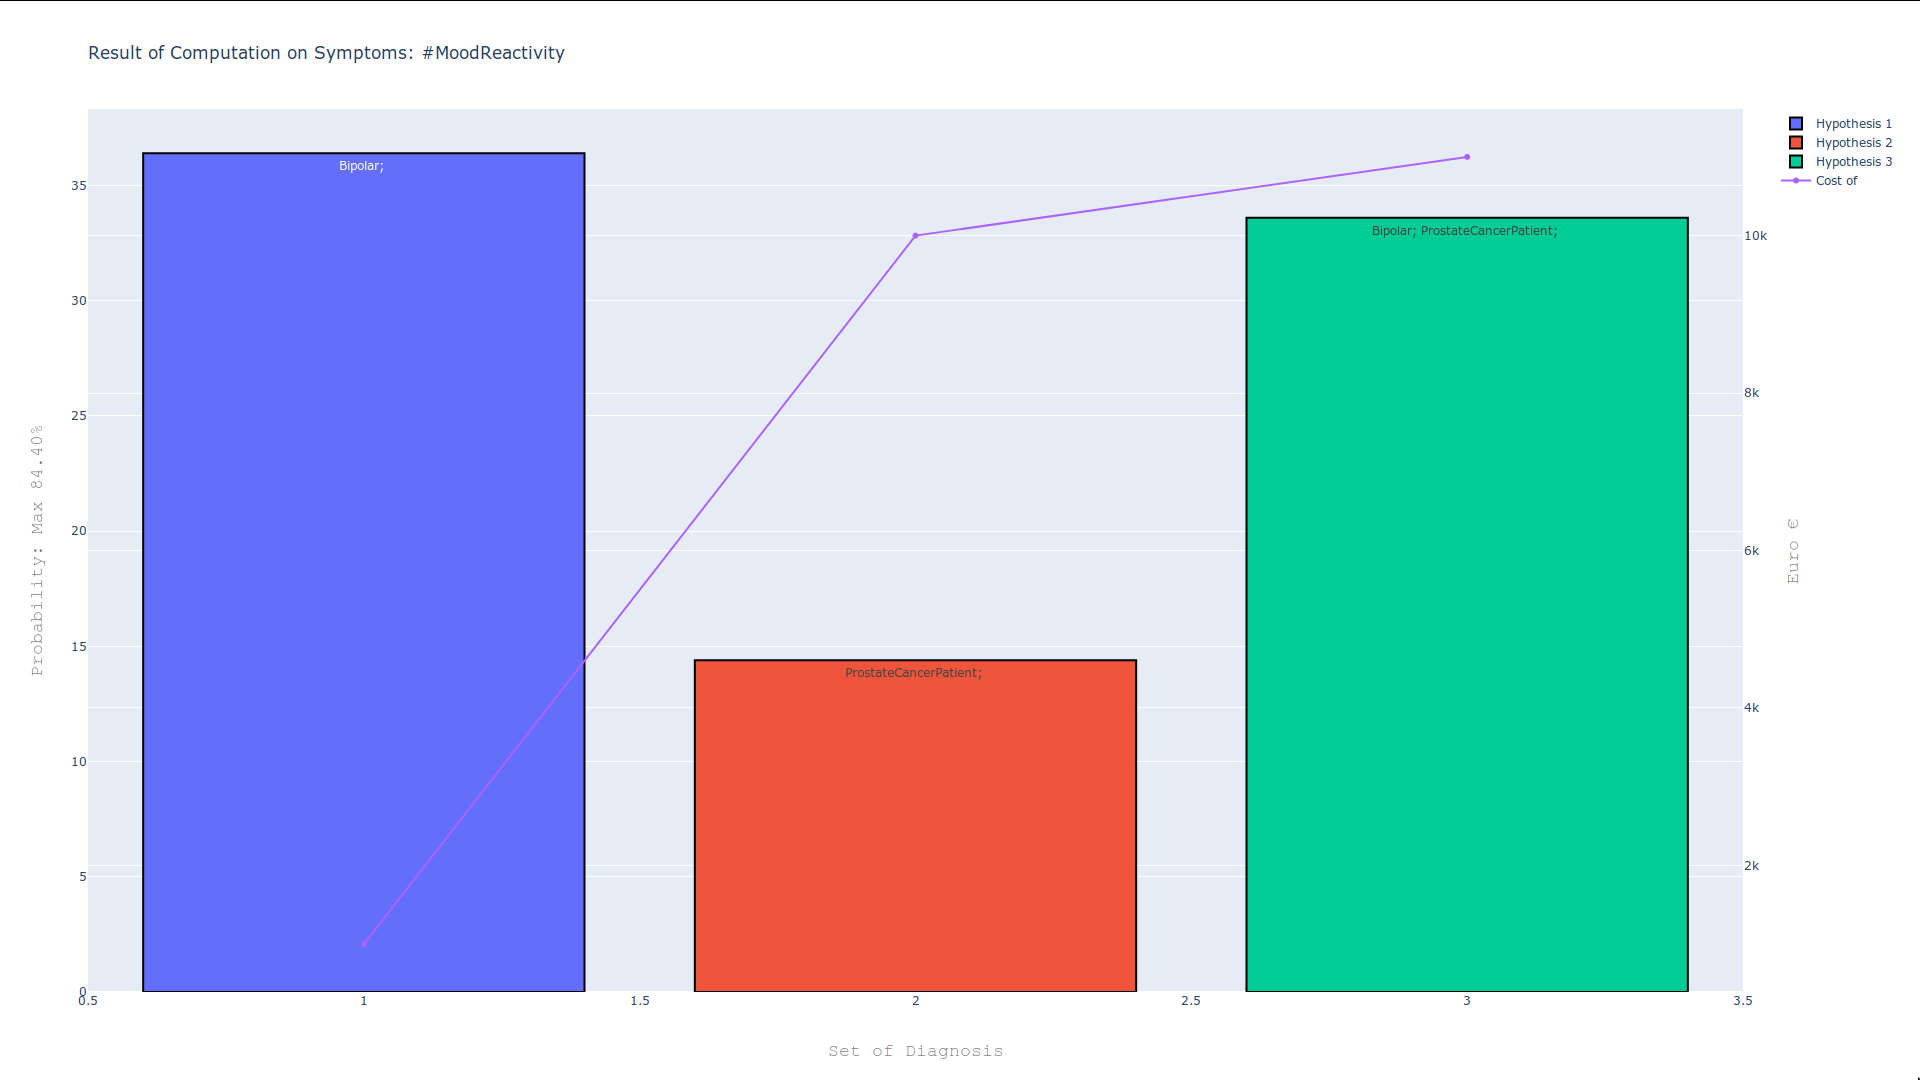
\includegraphics[width=\linewidth]{plot/Caso_di_studio.png}
	\caption{Versione Web}
	\label{fig: A_web}
\end{figure}

\begin{figure}
	\centering
	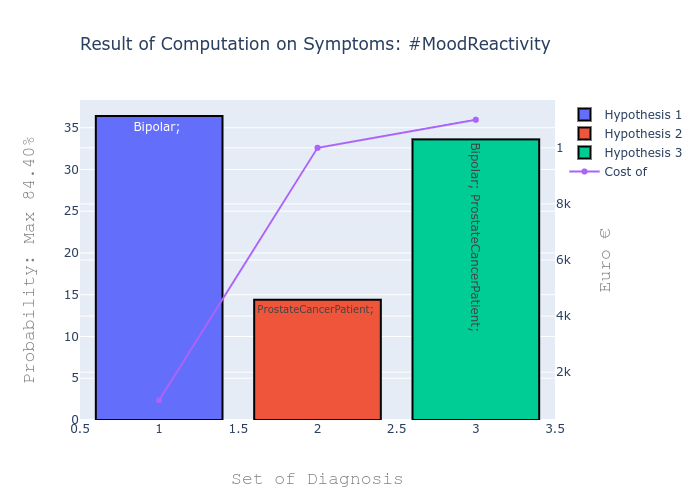
\includegraphics[width=\linewidth]{plot/caso_di_studio_alt.png}
	\caption{Versione documento}
	\label{fig: A_doc}
\end{figure}